% Chapter Template

\chapter{Development} % Main chapter title

\label{Chapter3} % Change X to a consecutive number; for referencing this chapter elsewhere, use \ref{ChapterX}

\section{Problem Statement}
The goal of this project is to create a system with a better scalability and reliability compared to the existing EPIC infrastructure using a container-orchestrated infrastructure while improving our development cycle by switching to a microservices architecture. In addition to improve real time query flexibility and overall performance.

\section{Approach}

Container orchestrated systems help deploy microservices architectures as well as abstract their physical structure. They add a logical abstraction on top of the physical structure allows to work independently from the underneath infrastructure, which makes it easier to move between different cloud infrastructures.

In addition, microservice architectures make systems more flexible as they decouple between functionalities, making it easier and more cost efficient to replace tools and evolve the system.  We will take an asynchronous/choreography approach for microservices with message queuing systems. This approach decreases coupling between components increasing the capability to add new components without having to change any configuration.

We will design the system to fit and take advantage of container orchestrated technology. This systems make it easy to create infrastructure on demand. Which in turn would allow for a better optimization of resources. One improvement of the “on demand” feature, is the ability to modify infrastructure on state change. Which in that sense would make possible to remove the state from the designed microservices, make them unaware of the state changes. Thanks to this capability we can design microservices that are completely stateless, improving the performance by removing responsibilities and making their development  and maintenance easier.

As we have previously seen, the current EPIC infrastructure use cases can be summarized in 4 points:

\begin{itemize}
	\item Collect tweets in real time
	\item Classify collected tweets in real time
	\item Modify classification in real time
	\item Analyze collected data
\end{itemize}


In that way, we first need a place to store tweets. To store tweets we use Cassandra as it’s the one used by the current EPIC infrastructure. Currently Cassandra is the best option thanks to it’s write perfomance, high scalability and great concurrency. In addition, it’s backed by DataStax a private company that has written a high amount of documentation in how to optimize Cassandra deployments.

To collect the data in real time, we need a microservice that connects to the public Twitter API and requests tweets. For that we use the Streaming API. We create a specific microservice for this. In order to remember it later, we will call it Twitter tracker. It will act as a gateway pulling data from the public API and passing it to the messaging system to be processed. We just want to get the tracked tweets into the system.

To classify the incoming data, we can take advantage of the orchestration system and create an instance for each category we need to store. We plug each instance into the queue created by Twitter tracker and make that each instance decides if each message is part of their own category or not. If the answer is positive, this microservice will store the tweet as well as normalize it. This way, we have normalized tweets which in turn will make it easier to analyze the data that we have. We will call this microservice Tweet normalizer. For each category we will have an instance running. As we previously stated, this makes the microservice way easier to develop.

Next, we need to modify and create the classification configuration in real time. To do so, we would need a couple of components:

\begin{itemize}
	\item \textit{Event Manager UI}: Let’s analysts manage categories/events adding keywords, toggling tracking and more. This microservice would not manage anything from the system, it would be completely unaware of the surrounding system where it is running and what other microservices exist. Finally, any change performed in the state will be broadcasted through a messaging system so that any other microservice can act upon the change. Messages should contain full state instead of incremental states. This is to ensure that state storage responsibility is not replicated in differents components. 
	\item \textit{Infrastructure Controller}:  Subscribes to the messages generated for events and modifies the current infrastructure creating or destroying instances of tweet normalizer or updating \textit{Twitter tracker}  in order to match the change. This microservice needs to be aware of the orchestration system where its running. However, thanks to the \textit{Event Manager UI} sending messages with full state, we can make this component totally stateless. In addition, the responsibility of detecting what changes need to be performed in the infrastructure can stay into the container orchestrated system. So this microservice responsibility stays limited to translating changes in state to changes in infrastructure

\end{itemize}

Finally, Analysts want to access the collected data and perform analysis on top of it. Cassandra is not really prepared to answer specific queries from analysts. Its CQL interface is great for small queries but doesn’t allow for high complexity. In addition, it was never intended to be used as an analysis tool. So we choose a different tool that it's optimized to read and process large datasets: Spark. It is a well known big data processing tool, and it has a connector for Cassandra that takes advantage of the cluster data locality to perform tasks. This way we take the read aspect of the cluster away from Cassandra and give to a tool that has been optimized for this task.In order to make it easier for analysts to access and perform analysis, we will add a web Notebook UI to give analysts an easy way to execute queries on Spark with a web UI.

\begin{figure}
\centering
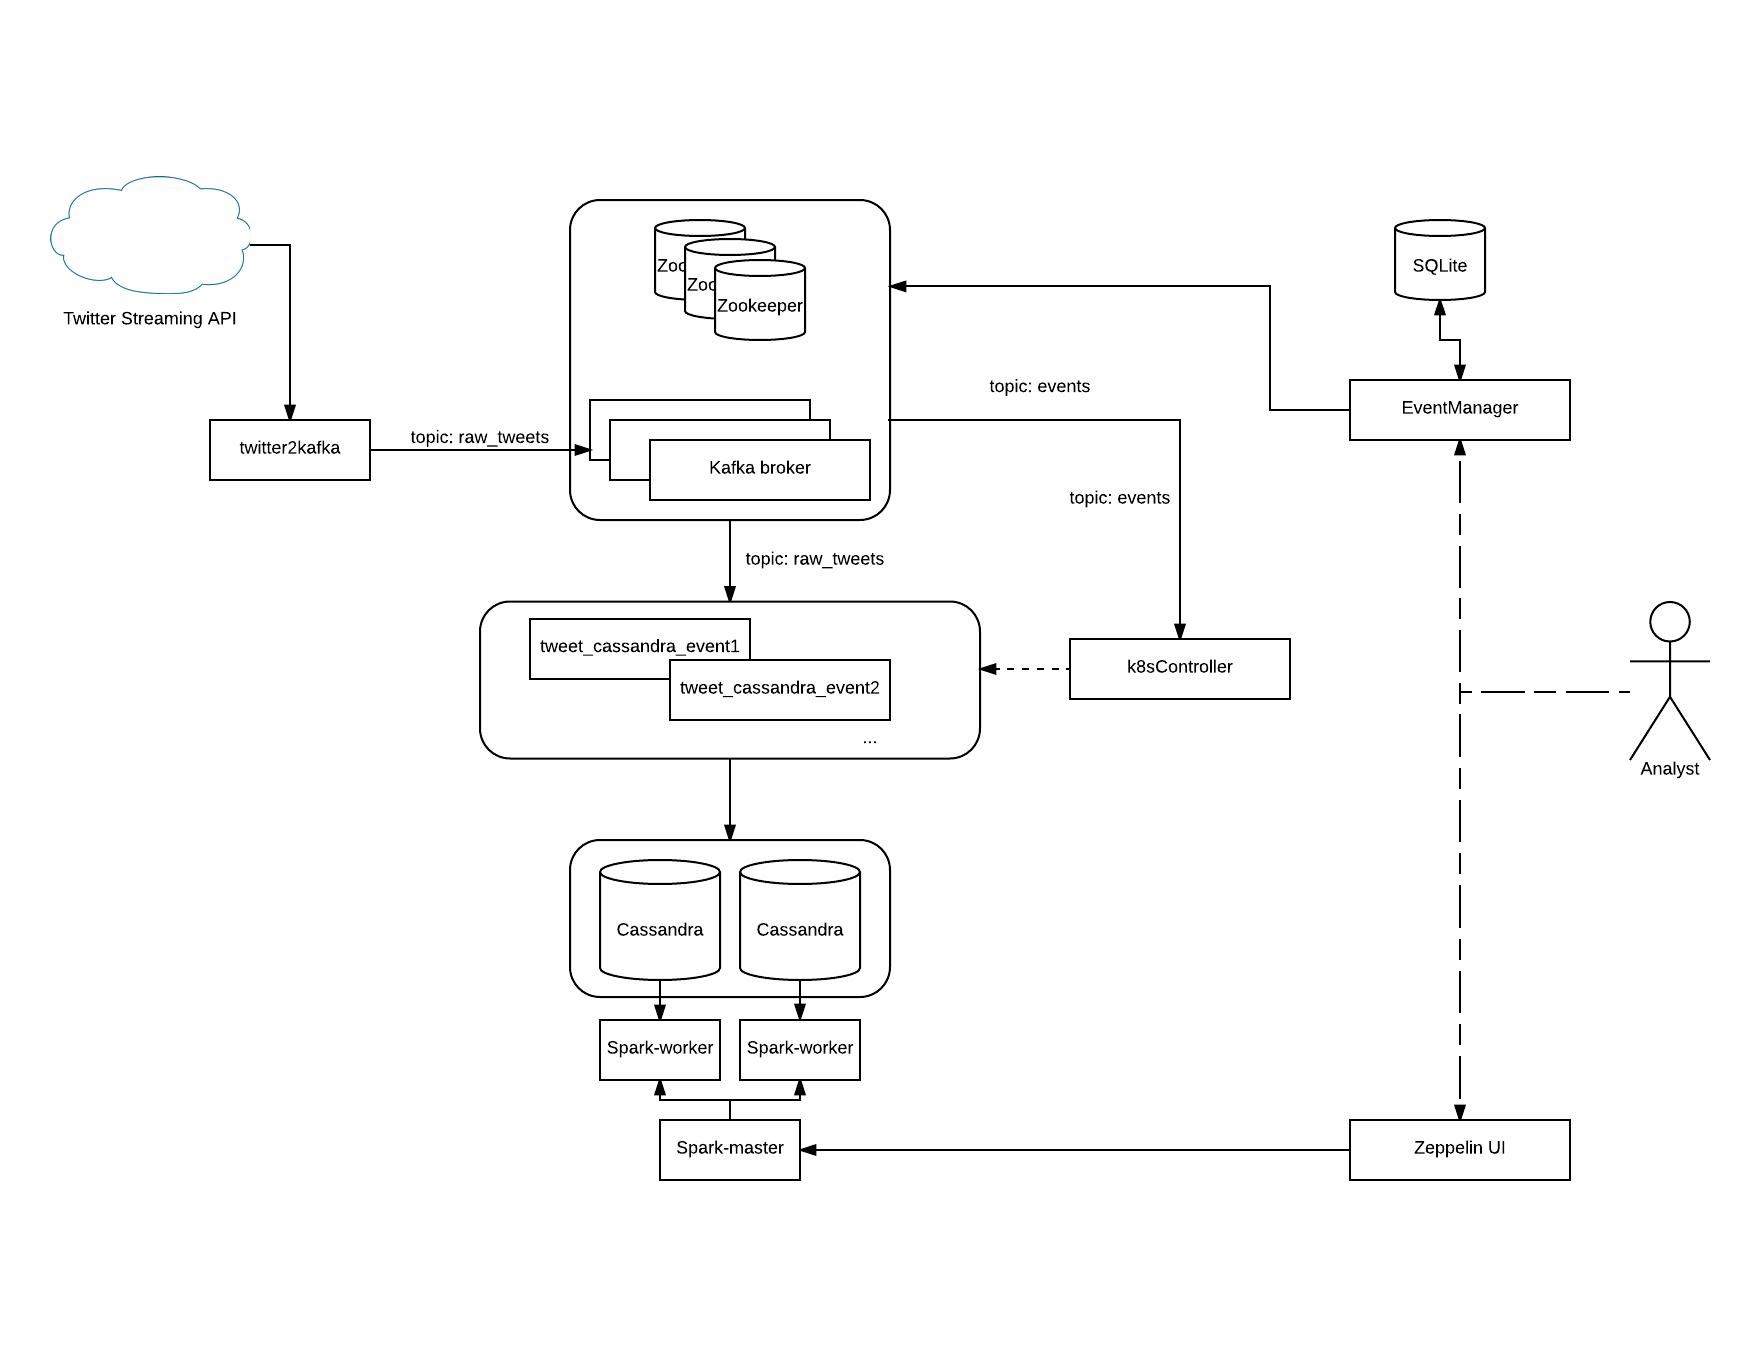
\includegraphics[width=\textwidth]{Figures/SysArch}
\decoRule
\caption[System architecture]{Proposed system architecture}
\label{fig:SysArch}
\end{figure}

\section{Implementation}

To prove that the specified architecture is feasible, I developed a working prototype of the system. 

We started with 2 nodes of Cassandra to store the tweets with Google Cloud disks attached to keep data persistent. In order to deploy this, we use stateful sets, Kubernetes objects designed to support stateful components and allow scalability. Persistent volumes can be attached to any node to keep data between restarts keeping a naming consistency. They can be used for stateful scalable apps like distributed databases. They provide an easy way to add or removed nodes from the set, allowing for a controlled scalability. In our case we could scale Cassandra dynamically to increase storage space and/or performance by making the cluster more parallel.

In addition, we add a spark workers to each instance of Cassandra to increase and ensure data locality when running Spark jobs. This way, spark works with local data from their correspondent Cassandra node. All of this workers are coordinated by a spark master node that is in charge of planning and distributing the work between each worker.

To interact with the Spark cluster, we deploy a Zeppelin notebook container. We tweaked this container to interact efficiently with our Spark and Cassandra stack by adding a default configuration to use the cassandra-spark library. Notebooks makes the system more accessible by abstracting how to execute scripts in Spark and allowing to present results in an easy format of a website.

\begin{figure}
\centering
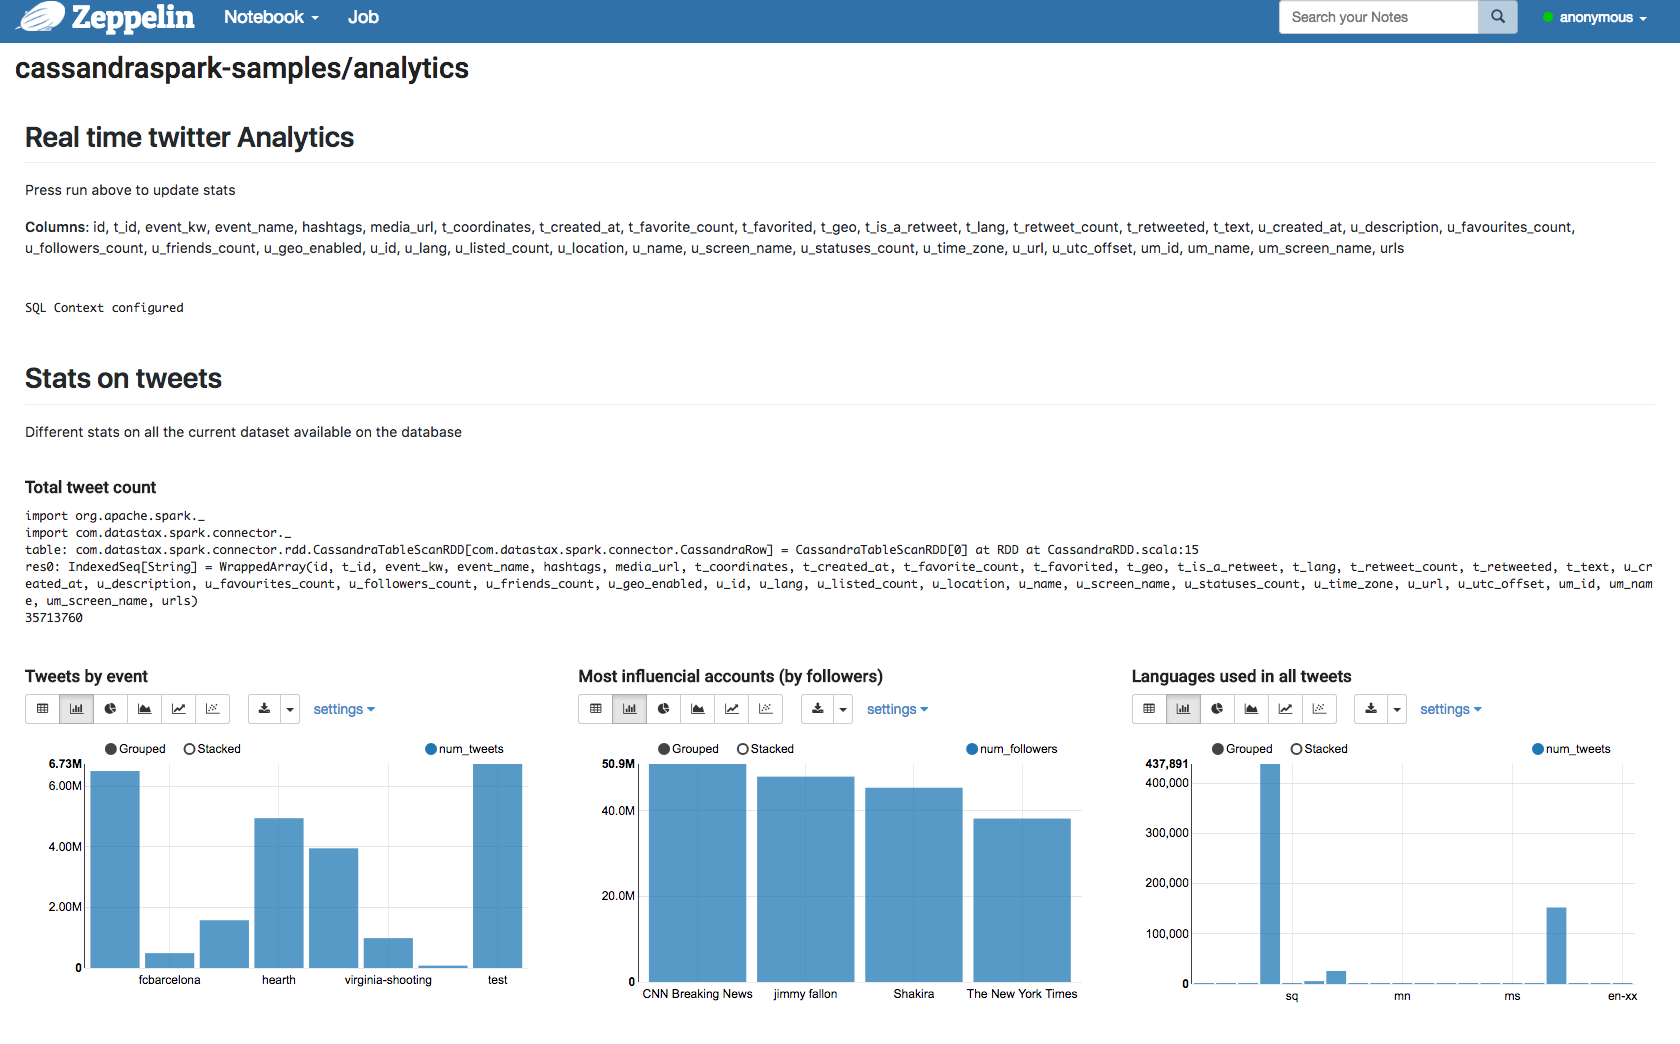
\includegraphics[width=\textwidth]{Figures/zeppelin}
\decoRule
\caption[Zeppelin visualization example]{Zeppelin server with some visualization from the dataset}
\label{fig:zeppelin}
\end{figure}

We also need some custom microservices for the designed solution. At the beginning all microservices were implemented in Python, basically because it’s easy and fast to prototype, and it also let’s use iterate faster. The goal was to keep all microservices short and simple in order to make their maintenance easy, enabling developers to maintain and deploy changes faster. Also, keeping them small makes it easy if any microservice needs to be rewritten in another language because python is not fast enough. Apart from implementing them, we also needed to containerize them to make deployment in the orchestration server easier. 


For the collection pipe, we divided the process to support better scalability and avoid high incoming tweets to collapse the system. Between parts we use Kafka a high reliable messaging system. Thanks to this decoupling we could also plug other backend to analyze tweets in real time. 

Finally, to make the system work we need to add a few custom components. The following components were implemented specially to work on the described environment. 

\begin{itemize}
	\item \textit{Tweet normalizer}: Fast classifier and tweet data normalizer that receives tweets from the raw\_tweets pipe and stores them on Cassandra. This microservice is designed to only keep track of one event. The tracked event information is sent to the microservice on start through environment variables defined with Kubernetes. To increase this microservice performance, some C based libraries replaced some regular Python libraries for intensive task as json encoding and loading. 
	\item \textit{Twitter tracker}: Twitter Streaming API client. Connects to the public Streaming API to fetch tweets and send them to the raw\_tweets pipe.  Written initially on Python and re-written in Go afterwards to increase throughput and avoid some python errors that appeared after a couple of days running.
	\item \textit{Event Manager UI}: Stateful django web application for analysts to interact with. Enables CRUD actions on events. Any change on state is later broadcasted to the rest of the system through Kafka. It keeps track of changes made on events to facilitate collaboration between analysts. SQLite as a file is used for storing data and a Google Cloud disk is used to allow saving state between container restarts.
	\item \textit{Infrastructure controller}: In this case this is a Kubernetes controller, written in python using a python client library. It subscribes to the Kafka topic and receives events generated by the event manager UI. It applies changes to the infrastructure incrementally to meet the changes performed in the UI by the analysts. It’s completely stateless, all it does is act upon what is received. 
\end{itemize}


\begin{figure}
\centering
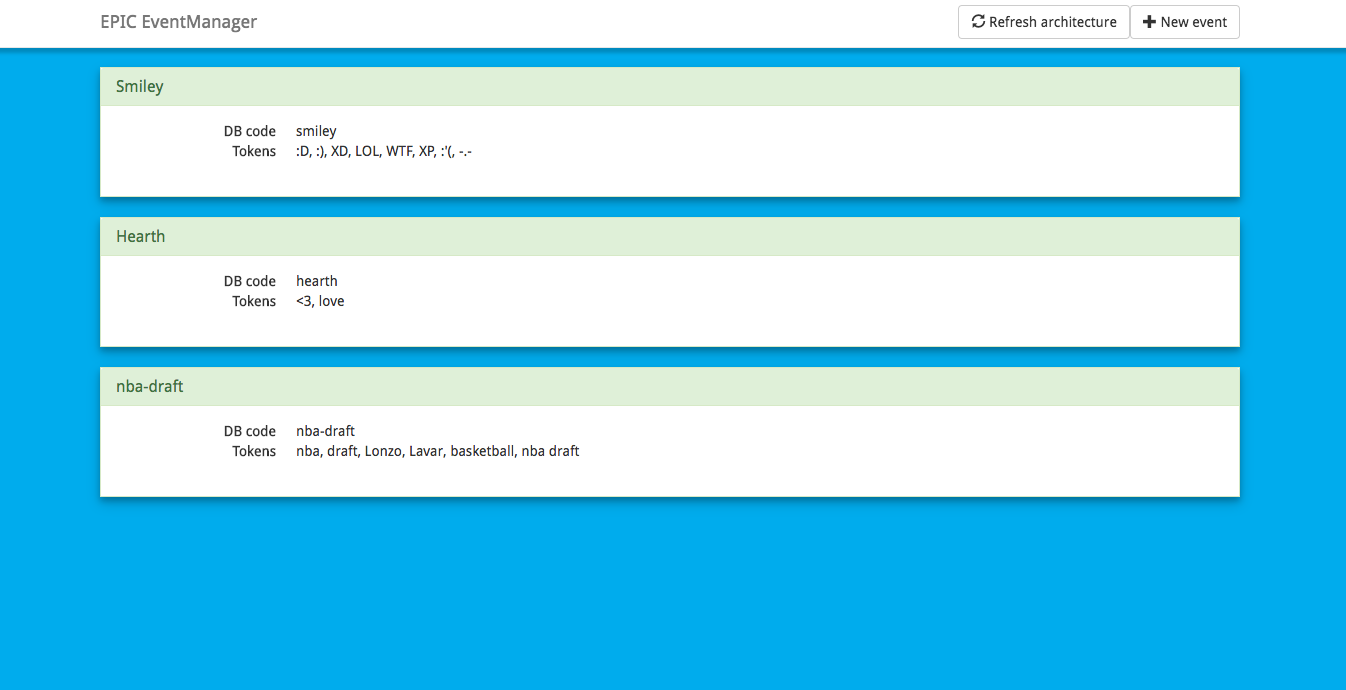
\includegraphics[width=\textwidth]{Figures/eventmanager}
\decoRule
\caption[Event Manager UI]{Event manager UI}
\label{fig:eventmanager}
\end{figure}

\subsection{Deployment}

To deploy the system, we create a 4 node cluster on Google Container engine. Each node having 1 virtual CPU and 4Gb or RAM. This is the major factor limiting our deployment. We also limit each Cassandra node to 1 GB of RAM for the Cassandra part. We won’t limit Spark, as we want it to use as much resources as we have available. 

To start we need to deploy the basic components driving the infrastructure. Those are Kafka and Cassandra. In our case we are running Kafka with 2 brokers and Cassandra with 3 nodes each one running Spark as a sidecar. After this we need to deploy the frontend components. One the analytics side we deploy Zeppelin, and on the collecting side we deploy the EventManager. The final part is the Kubernetes controller. Once deployed the rest of the infrastructure will be deployed when the state requires it.

Tracking will start once we add an event in the EventManager UI. After the creation action, the UI will send a message through Kafka saying that this event was created. Kubernetes Controller will collect this message and update the twitter tracker and will create a new microservice to normalize and classify tweets for the provided event.

